\documentclass[conference]{IEEEtran}
\newcommand*{\rootPath}{./}

\usepackage{url}

% math and cs
% \usepackage[]{algorithm2e}
\usepackage[linesnumbered,lined,boxed,commentsnumbered]{algorithm2e}
\usepackage{amsmath}
\usepackage{amssymb}
\usepackage{mathrsfs}
\newtheorem{definition}{Definition}
\newtheorem{proposition}{Proposition}
\newenvironment{proof}[1][Proof]{\begin{trivlist}
  \item[\hskip \labelsep {\bfseries #1}]}{\end{trivlist}}
  % \newenvironment{definition}[1][Definition]{\begin{trivlist}
  % \item[\hskip \labelsep {\bfseries #1}]}{\end{trivlist}}
  % \newenvironment{example}[1][Example]{\begin{trivlist}
  % \item[\hskip \labelsep {\bfseries #1}]}{\end{trivlist}}
  % \newenvironment{remark}[1][Remark]{\begin{trivlist}
  % \item[\hskip \labelsep {\bfseries #1}]}{\end{trivlist}}

% style
\usepackage{booktabs}
\usepackage{multirow}
\usepackage{lipsum}
\usepackage{todonotes}
\usepackage{standalone}
\usepackage{import}
\usepackage{url}
%\Urlmuskip=0mu plus 1mu %bug url

% graph
\usepackage{graphicx}
\usepackage[outdir=./]{epstopdf}
\usepackage[labelformat=simple]{subcaption}
\usepackage{array}
%\usepackage[colorinlistoftodos]{todonotes}
\newcommand{\HRule}{\rule{\linewidth}{0.5mm}}



\DeclareCaptionLabelSeparator{periodspace}{.\quad}
\captionsetup{font=footnotesize,labelsep=periodspace,singlelinecheck=false}
\captionsetup[sub]{font=footnotesize,singlelinecheck=true}


\usepackage[english,american]{babel}



\usepackage[capitalise,nameinlink]{cleveref}
%Nice formats for \cref
\crefname{section}{Sect.}{Sect.}
\Crefname{section}{Section}{Sections}
\crefname{figure}{Fig.}{Fig.}
\Crefname{figure}{Figure}{Figures}

\usepackage{xspace}
%\newcommand{\eg}{e.\,g.\xspace}
%\newcommand{\ie}{i.\,e.\xspace}
\newcommand{\eg}{e.\,g.,\ }
\newcommand{\ie}{i.\,e.,\ }


\renewcommand\thesubfigure{(\alph{subfigure})}


%invert table
\usepackage{collcell}
\usepackage{datatool}
\usepackage{environ}

%\newcolumntype{C}[1]{>{\centering}m{#1}}
%\newcolumntype{C}[1]{>{\centering\raggedright\arraybackslash}m{#1}}
\newcolumntype{L}[1]{>{\raggedright\let\newline\\\arraybackslash\hspace{0pt}}m{#1}}
\newcolumntype{C}[1]{>{\centering\let\newline\\\arraybackslash\hspace{0pt}}m{#1}}
\newcolumntype{R}[1]{>{\raggedleft\let\newline\\\arraybackslash\hspace{0pt}}m{#1}}
 
\standalonetrue

\title{Syst\`eme de vote sur la Primaire.org}
 
\author{
    \IEEEauthorblockN{Pierre-Louis Guhur, Thibauld Favre}
}


\begin{document}
  
  
\maketitle


\begin{abstract} 
LaPrimaire.org organise une primaire ouverte en France pour les \'elections pr\'esidentielles de 2017. Elle rel\`eve le d\'efi d'organiser un vote d\'emocratique avec plus d'une centaine de candidats. Le syst\'eme de vote pr\'esidentiel, appel\'e \emph{vote majoritaire} n'est pas adapt\'e \'a un tel vote. La raison principale est que tous les \'electeurs ne peuvent pas \'etudier attentivement chacun des candidats. En outre, le vote majoritaire comporte plusieurs inconv\'enients qui faussent la repr\'esentativit\'e du vote. LaPrimaire.org a donc developp\'e un nouveau syst\`eme de vote, bas\'e sur le Jugement Majoritaire. Plus sp\'ecifiquement, le vote se d\'eroule en deux phases, au cours desquelles un \'electeur attribut \`a chaque candidat un jugement Tr\`es bien, Bien, Assez bien, Correct ou D\'efavorable. Lors de la premi\'ere phase, les jugements ne sont exprim\'es que sur un lot de 10 candidats. Cet article montre comment construire ces lots et quel est le nombre minimum d'\'electeurs n\'ecessaires pour assurer la fiabilit\'e de ce syst\`eme de vote.
\end{abstract}



\documentclass[conference]{IEEEtran}
\newcommand*{\rootPath}{../}
\usepackage{url}

% math and cs
% \usepackage[]{algorithm2e}
\usepackage[linesnumbered,lined,boxed,commentsnumbered]{algorithm2e}
\usepackage{amsmath}
\usepackage{amssymb}
\usepackage{mathrsfs}
\newtheorem{definition}{Definition}
\newtheorem{proposition}{Proposition}
\newenvironment{proof}[1][Proof]{\begin{trivlist}
  \item[\hskip \labelsep {\bfseries #1}]}{\end{trivlist}}
  % \newenvironment{definition}[1][Definition]{\begin{trivlist}
  % \item[\hskip \labelsep {\bfseries #1}]}{\end{trivlist}}
  % \newenvironment{example}[1][Example]{\begin{trivlist}
  % \item[\hskip \labelsep {\bfseries #1}]}{\end{trivlist}}
  % \newenvironment{remark}[1][Remark]{\begin{trivlist}
  % \item[\hskip \labelsep {\bfseries #1}]}{\end{trivlist}}

% style
\usepackage{booktabs}
\usepackage{multirow}
\usepackage{lipsum}
\usepackage{todonotes}
\usepackage{standalone}
\usepackage{import}
\usepackage{url}
%\Urlmuskip=0mu plus 1mu %bug url

% graph
\usepackage{graphicx}
\usepackage[outdir=./]{epstopdf}
\usepackage[labelformat=simple]{subcaption}
\usepackage{array}
%\usepackage[colorinlistoftodos]{todonotes}
\newcommand{\HRule}{\rule{\linewidth}{0.5mm}}



\DeclareCaptionLabelSeparator{periodspace}{.\quad}
\captionsetup{font=footnotesize,labelsep=periodspace,singlelinecheck=false}
\captionsetup[sub]{font=footnotesize,singlelinecheck=true}


\usepackage[english,american]{babel}



\usepackage[capitalise,nameinlink]{cleveref}
%Nice formats for \cref
\crefname{section}{Sect.}{Sect.}
\Crefname{section}{Section}{Sections}
\crefname{figure}{Fig.}{Fig.}
\Crefname{figure}{Figure}{Figures}

\usepackage{xspace}
%\newcommand{\eg}{e.\,g.\xspace}
%\newcommand{\ie}{i.\,e.\xspace}
\newcommand{\eg}{e.\,g.,\ }
\newcommand{\ie}{i.\,e.,\ }


\renewcommand\thesubfigure{(\alph{subfigure})}


%invert table
\usepackage{collcell}
\usepackage{datatool}
\usepackage{environ}


\standalonetrue

\begin{document}

%%=============================================================================



\section{Introduction}
\label{sec:intro}

Les fran\c{c}ais sont majoritairement d\'efiants envers leurs politiques. 
Une \'etude men\'e par CEVIPOF \cite{cevipof2016} montre qu'en janvier 2016, $67\%$ des fran\c{c}ais pensent que la d\'emocratie ne fonctionne pas tr\`es bien voire pire. $76\%$ des fran\c{c}ais disent que les \'elu(e)s et les dirigeant(e)s politiques fran\c{c}ais sont plut\^ot corrompu(e)s. 

LaPrimaire.org est une solution citoyenne pour r\'epondre \`a cette d\'efiance. 
Notre m\'ethode est d'am\'eliorer la repr\'esentativit\'e de la soci\'et\'e fran\c{c}aise. Pour cela, nous organisons une primaire pr\'esidentielle pour les \'elections de 2017 en France dans laquelle chaque citoyen fran\c{c}ais peut candidater. L'\'elu(e) recevra un soutien financier, l\'egal et les 500 signatures d'\'elus provenant de 30 d\'epartements diff\'erents avec 50 \'elus maximum par d\'epartement.

Pour faciliter l'apparition de nouveaux repr\'esentants, la Primaire repose sur plusieurs principes, comme indiqu\'es dans son manifeste~\cite{manifeste}: elle n'est pas un parti politique ; elle n'a pas de programme politique ; un candidat n'est pas jug\'e sur sa notori\'et\'e mais sur ses id\'ees.

Le syst\`eme de vote actuellement utilis\'e pour les \'elections pr\'esidentielles, appel\'e \emph{vote majoritaire}, va au contraire du principe de notori\'et\'e. Par exemple, il serait facile pour un chanteur de demander \'a ses fans de s'inscrire sur laPrimaire.org. Il disposerait alors d'un plus grand nombre de votes qu'un citoyen ordinaire. Le vote majoritaire souffre d'autres inconv\'enients qui d\'efavorisent la repr\'esentativit\'e, comme present\'e dans la \cref{sec:mv}. 

C'est pour cela que nous nous sommes tourn\'es vers un nouveau syst\`eme de vote, appel\'e jugement majoritaire (JM). Le principe de ce syst\`eme est de juger chaque candidat selon un bar\^eme de mentions: tr\`es bien, bien, assez bien, correct et d\'evaforable. Le gagnant d'une \'election est alors celui qui rassemble les meilleurs mentions au sens de la m\'edianne.  Le JM a \'et\'e propos\'e pour la premi\'ere fois par deux chercheurs fran\c{c}ais, Michel Balinski et Rida Laraki \cite{balinski2010majority}.  Il a \'et\'e test\'e lors des \'elections pr\'esidentielles de 2012 par un sondage command\'e par le \emph{think tank} Terra Nova  et r\'ealis\'e par l'institut OpinionWay aupr\`es d'un \'echantillon repr\'esentatif de 1034 personnes \cite{balinski2012rendre}. Dans la \cref{sec:mj}, nous r\'esumons ses avantages et inconv\'enients par rapport \`a d'autres syst\`emes de vote. 

Si ce syst\`eme permet d'am\'eliorer la repr\'esentativit\'e du vote, il n'est pas con\c{c}u pour fonctionner avec un grand nombre de candidats. Tous les \'electeurs ne peuvent pas \'etudier de mani\`ere approfondie plus de 100 candidats. Par soucis pratique, les candidats ayant de plus de notori\'et\'e m\'ediatique seraient encore avantag\'es. C'est pourquoi, nous avons deriv\'e le JM pour l'adapter \`a un grand nombre de candidats. Plus concr\`etement,
le vote se d\'eroule en deux phases. Au cours de la premi\`ere phase, chaque \'electeur s'exprime seulement sur un lot de candidats pour qualifier les meilleurs candidats. Lors de la seconde phase, les \'electeurs s'expriment sur ces candidats qualifi\'es.
Dans la \cref{sec:laprimaire}, nous montrons que comment notre proc\'ed\'e pour construire un lot permet d'assurer l'\'equir\'epartie entre les candidats. En se basant sur les r\'esultats du sondage OpinionWay/Terra Nova, nous avons extrapol\'e des r\'esultats de vote sur un nombre variable de candidats, puis simul\'e des \'elections. Cela a permis d'\'etablir le nombre minimum d'\'electeurs n\'ecessaire \`a rendre le vote fiable selon le nombre de candidats.



\end{document}




\documentclass[conference]{IEEEtran}
\newcommand*{\rootPath}{../}
\usepackage{url}

% math and cs
% \usepackage[]{algorithm2e}
\usepackage[linesnumbered,lined,boxed,commentsnumbered]{algorithm2e}
\usepackage{amsmath}
\usepackage{amssymb}
\usepackage{mathrsfs}
\newtheorem{definition}{Definition}
\newtheorem{proposition}{Proposition}
\newenvironment{proof}[1][Proof]{\begin{trivlist}
  \item[\hskip \labelsep {\bfseries #1}]}{\end{trivlist}}
  % \newenvironment{definition}[1][Definition]{\begin{trivlist}
  % \item[\hskip \labelsep {\bfseries #1}]}{\end{trivlist}}
  % \newenvironment{example}[1][Example]{\begin{trivlist}
  % \item[\hskip \labelsep {\bfseries #1}]}{\end{trivlist}}
  % \newenvironment{remark}[1][Remark]{\begin{trivlist}
  % \item[\hskip \labelsep {\bfseries #1}]}{\end{trivlist}}

% style
\usepackage{booktabs}
\usepackage{multirow}
\usepackage{lipsum}
\usepackage{todonotes}
\usepackage{standalone}
\usepackage{import}
\usepackage{url}
%\Urlmuskip=0mu plus 1mu %bug url

% graph
\usepackage{graphicx}
\usepackage[outdir=./]{epstopdf}
\usepackage[labelformat=simple]{subcaption}
\usepackage{array}
%\usepackage[colorinlistoftodos]{todonotes}
\newcommand{\HRule}{\rule{\linewidth}{0.5mm}}



\DeclareCaptionLabelSeparator{periodspace}{.\quad}
\captionsetup{font=footnotesize,labelsep=periodspace,singlelinecheck=false}
\captionsetup[sub]{font=footnotesize,singlelinecheck=true}


\usepackage[english,american]{babel}



\usepackage[capitalise,nameinlink]{cleveref}
%Nice formats for \cref
\crefname{section}{Sect.}{Sect.}
\Crefname{section}{Section}{Sections}
\crefname{figure}{Fig.}{Fig.}
\Crefname{figure}{Figure}{Figures}

\usepackage{xspace}
%\newcommand{\eg}{e.\,g.\xspace}
%\newcommand{\ie}{i.\,e.\xspace}
\newcommand{\eg}{e.\,g.,\ }
\newcommand{\ie}{i.\,e.,\ }


\renewcommand\thesubfigure{(\alph{subfigure})}


%invert table
\usepackage{collcell}
\usepackage{datatool}
\usepackage{environ}


\standalonetrue

\begin{document}

%%=============================================================================



\section{Le vote majoritaire}
\label{sec:mv}

\subsection{Le paradoxe de Condorcet}

\subsection{Les strat\'egies partisannes}

\end{document}



\documentclass[conference]{IEEEtran}
\newcommand*{\rootPath}{../}
\usepackage{url}

% math and cs
% \usepackage[]{algorithm2e}
\usepackage[linesnumbered,lined,boxed,commentsnumbered]{algorithm2e}
\usepackage{amsmath}
\usepackage{amssymb}
\usepackage{mathrsfs}
\newtheorem{definition}{Definition}
\newtheorem{proposition}{Proposition}
\newenvironment{proof}[1][Proof]{\begin{trivlist}
  \item[\hskip \labelsep {\bfseries #1}]}{\end{trivlist}}
  % \newenvironment{definition}[1][Definition]{\begin{trivlist}
  % \item[\hskip \labelsep {\bfseries #1}]}{\end{trivlist}}
  % \newenvironment{example}[1][Example]{\begin{trivlist}
  % \item[\hskip \labelsep {\bfseries #1}]}{\end{trivlist}}
  % \newenvironment{remark}[1][Remark]{\begin{trivlist}
  % \item[\hskip \labelsep {\bfseries #1}]}{\end{trivlist}}

% style
\usepackage{booktabs}
\usepackage{multirow}
\usepackage{lipsum}
\usepackage{todonotes}
\usepackage{standalone}
\usepackage{import}
\usepackage{url}
%\Urlmuskip=0mu plus 1mu %bug url

% graph
\usepackage{graphicx}
\usepackage[outdir=./]{epstopdf}
\usepackage[labelformat=simple]{subcaption}
\usepackage{array}
%\usepackage[colorinlistoftodos]{todonotes}
\newcommand{\HRule}{\rule{\linewidth}{0.5mm}}



\DeclareCaptionLabelSeparator{periodspace}{.\quad}
\captionsetup{font=footnotesize,labelsep=periodspace,singlelinecheck=false}
\captionsetup[sub]{font=footnotesize,singlelinecheck=true}


\usepackage[english,american]{babel}



\usepackage[capitalise,nameinlink]{cleveref}
%Nice formats for \cref
\crefname{section}{Sect.}{Sect.}
\Crefname{section}{Section}{Sections}
\crefname{figure}{Fig.}{Fig.}
\Crefname{figure}{Figure}{Figures}

\usepackage{xspace}
%\newcommand{\eg}{e.\,g.\xspace}
%\newcommand{\ie}{i.\,e.\xspace}
\newcommand{\eg}{e.\,g.,\ }
\newcommand{\ie}{i.\,e.,\ }


\renewcommand\thesubfigure{(\alph{subfigure})}


%invert table
\usepackage{collcell}
\usepackage{datatool}
\usepackage{environ}


\standalonetrue

\begin{document}

%%=============================================================================



\section{Le jugement majoritaire}
\label{sec:mj}

Le jugement majoritaire (JM) a \'et\'e developp\'e par Balinski et Laraki \cite{mj} pour proposer une alternative au vote majoritaire. Nous pr\'esentons succinctement son fonctionnement, ses avantages et inconv\'enients. Pour plus de d\'etails, le lecteur est invit\'e \`a lire les articles mis en r\'ef\'erence.


\subsection{Fonctionnement}

Le JM demande \`a chaque \'electeur de juger chaque candidat selon au moins 5 mentions: Tr\`es bien, Bien, Assez bien, Correct et D\'efavorable. Lorsque tous les jugements ont \'et\'e exprim\'es, la m\'edianne des jugements de chaque candidat est calcul\'ee. En partant du meilleur jugement (ou du pire, a verifier), la m\'edianne est la mention pour laquelle le nombre de mentions sup\'erieures est \'egal au nombre de mentions inf\'erieures. Par exemple, si un candidat A a les mentions: Tr\`es bien, Tr\`es bien, Assez bien, Correct et D\'efavorable, son r\'esultat sera Assez bien. 

En cas d'\'egalit\'e entre deux candidats A et B, une proc\'edure appel\'ee \emph{algorithme de tie-breaking} permet de trouver le gagnant entre les deux candidats. Cette proc\'edure consiste \`a retirer les mentions m\'ediannes de A et B jusqu'\`a ce qu'elles diff\`erent. Par exemple, si le candidat B a les mentions: Tr\`es bien, Assez bien, Assez bien, Correct et D\'efavorable, alors A et B ont les m\^emes mentions m\'ediannes Assez bien. On retire alors momentan\'ement cette mention pour d'\'epartager A et B. A a alors les mentions: Tr\`es bien, Tr\`es bien, Correct et D\'efavorable. Sa mention m\'edianne est d\'esormais Tr\'es bien. En revanche, B a les mentions Tr\`es bien, Assez bien, Correct et D\'efavorable. Sa mention m\'edianne reste Assez bien. C'est pourquoi, B est class\'e apr\'es A. Si B avait toujours la m\^eme mention que A, on aurait continu\'e la proc\'edure en retirant une nouvelle fois (et jusqu'\`a ce que A se d\'epartage de B) la mention m\'edianne.

\subsection{Avantages}

Cette mani\`ere de voter rassemble de nombreux avantages qui justifient l'utilisation de ce syst\`eme de vote par rapport au vote majoritaire.



\subsection{Inconv\'enients}

Comme tous les syst\`emes de vote, il comporte \'egalement plusieurs inconv\'enients que nous ne jugeons pas probl\'ematique pour la primaire.

\end{document}




\documentclass[conference]{IEEEtran}
\newcommand*{\rootPath}{../}
\usepackage{url}

% math and cs
% \usepackage[]{algorithm2e}
\usepackage[linesnumbered,lined,boxed,commentsnumbered]{algorithm2e}
\usepackage{amsmath}
\usepackage{amssymb}
\usepackage{mathrsfs}
\newtheorem{definition}{Definition}
\newtheorem{proposition}{Proposition}
\newenvironment{proof}[1][Proof]{\begin{trivlist}
  \item[\hskip \labelsep {\bfseries #1}]}{\end{trivlist}}
  % \newenvironment{definition}[1][Definition]{\begin{trivlist}
  % \item[\hskip \labelsep {\bfseries #1}]}{\end{trivlist}}
  % \newenvironment{example}[1][Example]{\begin{trivlist}
  % \item[\hskip \labelsep {\bfseries #1}]}{\end{trivlist}}
  % \newenvironment{remark}[1][Remark]{\begin{trivlist}
  % \item[\hskip \labelsep {\bfseries #1}]}{\end{trivlist}}

% style
\usepackage{booktabs}
\usepackage{multirow}
\usepackage{lipsum}
\usepackage{todonotes}
\usepackage{standalone}
\usepackage{import}
\usepackage{url}
%\Urlmuskip=0mu plus 1mu %bug url

% graph
\usepackage{graphicx}
\usepackage[outdir=./]{epstopdf}
\usepackage[labelformat=simple]{subcaption}
\usepackage{array}
%\usepackage[colorinlistoftodos]{todonotes}
\newcommand{\HRule}{\rule{\linewidth}{0.5mm}}



\DeclareCaptionLabelSeparator{periodspace}{.\quad}
\captionsetup{font=footnotesize,labelsep=periodspace,singlelinecheck=false}
\captionsetup[sub]{font=footnotesize,singlelinecheck=true}


\usepackage[english,american]{babel}



\usepackage[capitalise,nameinlink]{cleveref}
%Nice formats for \cref
\crefname{section}{Sect.}{Sect.}
\Crefname{section}{Section}{Sections}
\crefname{figure}{Fig.}{Fig.}
\Crefname{figure}{Figure}{Figures}

\usepackage{xspace}
%\newcommand{\eg}{e.\,g.\xspace}
%\newcommand{\ie}{i.\,e.\xspace}
\newcommand{\eg}{e.\,g.,\ }
\newcommand{\ie}{i.\,e.,\ }


\renewcommand\thesubfigure{(\alph{subfigure})}


%invert table
\usepackage{collcell}
\usepackage{datatool}
\usepackage{environ}


\standalonetrue

\begin{document}

%%=============================================================================




\section{Notre syst\`eme de vote}
\label{sec:laprimaire}

Le syst\'eme de vote utilis\'e sur laPrimaire.org part du syst\`eme de vote du JM. Ce syst\`eme n'est pas adapt\'e pour un grand nombre de candidats, puisque tous les \'electeurs ne peuvent pas passer autant de temps \`a juger chaque candidat par soucis de temps.

\subsection{Fonctionnement}
L'\'election se d\'eroule en deux phases. Lors de la premi\`ere phase, les \'electeurs devront juger seulement un lot de 10 candidats, plut\^ot que de s'exprimer sur chaque candidat. Le nombre de 10 candidats correspond \`a la moyenne du nombre de candidats aux \'elections pr\'esidentielles depuis la r\'eforme du vote en 1962.

A l'issue de ce scrutin, les cinq candidats les mieux class\'es seront qualifi\'es. Nous avons choisi le chiffre cinq pour repr\'esenter plus de tendances politiques que lors du second tour aux \'elections pr\'esidentielles. 

Nous avons ajout\'e un quorum \`a la qualification: pour chaque candidat qualifi\'e, la moiti\'e de ses jugements ne doit pas \^etre D\'efavorable. Ce quorum sert \`a disqualifier les candidats trop clivants. Le seuil de $50\%$ a \'et\'e plac\'e haut pour d\'ecourager des strat\'egies de disqualifications. Par exemple si le seuil \'etait \`a $5\%$, les soutiens d'un candidat pourraient plus facilement s'unir pour disqualifier un autre candidat.

Lors de la seconde phase, les \'electeurs pourront juger pour tous les candidats qualifi\'es \`a l'aide du jugement majoritaire.


\subsection{Proc\'edure pour construire les lots}

Pour ne pas truquer la phase de qualification, les lots de 10 candidats sont choisis \'a l'avance et les \'electeurs ne pourront pas choisir les candidats qu'ils jugeront lors du premier tour. Pour que cette phase ne soit pas truqu\'ee, trois conditions ont \'et\'e s\'electionn\'ees.

\begin{enumerate}
  \item \emph{Le nombre d'apparition de chaque candidat dans les lots est le m\^eme.} Pour le vote majoritaire, ne pas apparaitre le m\^eme nombre de fois cr\'e\'e un biais important : si un candidat A re\c{c}oit $100\%$ des votes, mais n'apparait que dans $10\%$ des lots, il perdera contre un candidat B qui ne re\c{c}oit que $20\%$ des votes, mais qui apparait dans $100\%$ des lots. En revanche, ne pas recevoir strictement le m\^eme nombre de jugements n'influe pas sur le classement g\'en\'eral gr\^ace \`a l'utilisation de la m\'edianne.
  \item \emph{Chaque candidat a la m\^eme probabilit\'e de rencontrer tout autre candidat dans un lot.} Un biais cognitif dans les jugements consiste \`a juger un candidat par rapport \`a un autre : lorsqu'un \'electeur juge un candidat, il se r\'ef\`ere aux jugements qu'il a exprim\'e pr\'ec\'edemment. 
  \item Le classement est le m\^eme que si tous les \'electeurs jugent attentivement et ind\'ependemment chaque candidat. 
\end{enumerate}

Ces conditions sont d'autant plus difficiles \`a respecter que le nombre d\'electeurs n'est pas connu \`a l'avance : les \'electeurs peuvent s'inscrire \`a l'\'election, mais finalement ne pas y participer. Ainsi, une construction au pr\'ealable des lots n'est pas possible: si tous les \'electeurs devant s'exprimer sur un candidat ne sont pas pr\'esents lors de l'\'elections, alors ce candidat ne recevrait pas de jugements.


C'est pourquoi, la construction des lots se fait pendant le vote. Nous avons test\'e la proc\'edure suivante qui donne de bons r\'esultats:
Pour chaque lot, la proc\'edure consiste \`a :
\begin{enumerate}
  \item compter le nombre d'occurences $\#occ_i$ pour chaque candidat $i$ dans les lots pr\'ec\'edents ;
  \item construire un tableau qui attribut \`a candidat $i$ la valeur $1/\#occ_i$ si $\#occ_i \ne 0$ et $1$ sinon ;
  \item normaliser ce tableau en le divisant par la somme de chacune de ses cases ;
  \item ce tableau forme la probabilit\'e qu'\`a un candidat d'\^etre choisi dans le prochain lot.
\end{enumerate}

\subsection{Validation des deux premi\'eres contraintes}

\begin{figure*}[!ht]
  \centering
  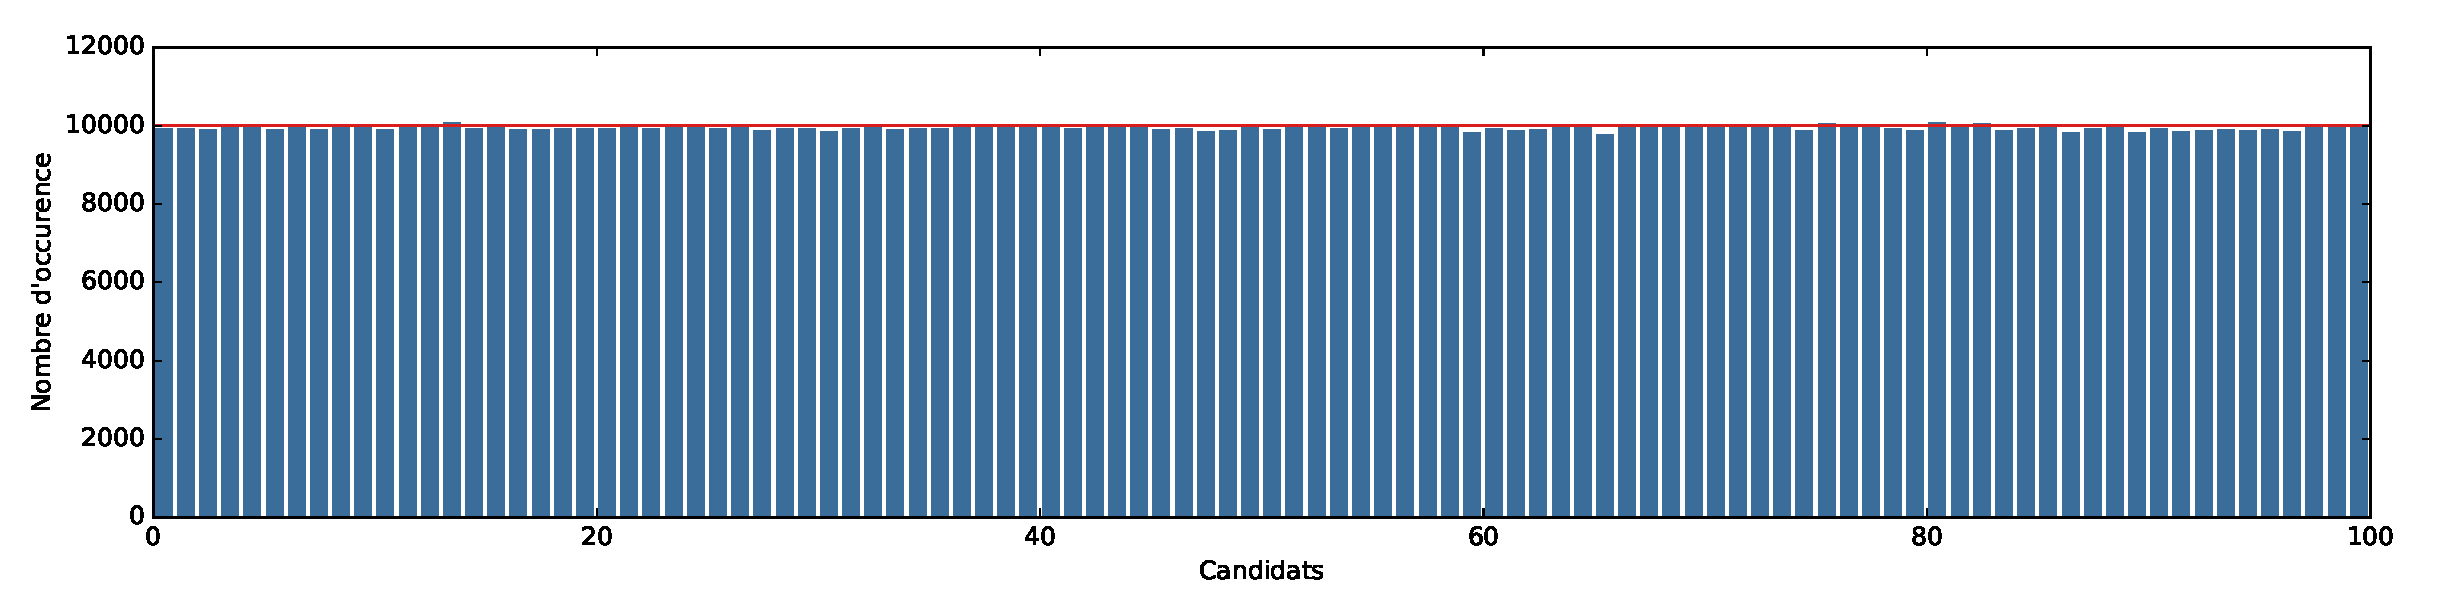
\includegraphics[width=0.98\textwidth]{../\rootPath image/lot_Nc-100_Ne-100000_Nl-10.pdf}
  \caption{Avec 100000 \'electeurs et 100 candidats, chaque candidat apparait autant de fois que les autres candidats dans les lots}
  \label{fig:candidatsVSoccurence}
\end{figure*}

Sur la \cref{fig:candidatsVSoccurence}, le nombre d'apparition de chaque candidat est repr\'esent\'e. Une ligne rouge repr\'esente la moyenne d'apparition. Chaque candidat n'apparait pas exactement le m\^eme nombre de fois, bien que l'\'ecart \`a la moyenne est visiblement faible. 

L'\'ecart-type est d\'efini comme la moyenne des \'ecarts \`a la moyenne. Il d\'epend du nombre d\'electeurs : plus les \'electeurs sont nombreux, et plus l'\'ecart-type devient faible. L'\'ecart-type seul est difficile \`a interpr\'eter : un \'ecart-type de 1 et une moyenne de 10 signifient qu'en g\'en\'eral, le nombre d'apparition d'un candidat est entre 9 ou 11. Avec une moyenne  de 10000, le nombre d'apparition d'un candidat est souvent entre 9999 et 10001 ; l'erreur est dans ce cas bien plus faible. En revanche, le rapport \'ecart-type sur moyenne est en revanche plus facile \`a interpr\'eter car il correspond \`a un pourcentage de d\'eviation. Dans nos tests, ce rapport est calcul\'e pour plusieurs tranches d\'electeurs. A partir de 30 000 \'electeurs, ce rapport devient inf\'erieur \`a $1\%$. Autrement dit, l'\'ecart dans le nombre d'apparition de chaque candidat est n\'egligeable.
La premi\`ere condition est donc valid\'ee. 

Pour valider la seconde condition, nous avons compt\'e le nombre de fois qu'un candidat rencontre un autre candidat dans un m\^eme lot. Avec 30 000 \'electeurs, le rapport entre l'\'ecart-type et la moyenne de ce nombre est inf\'erieur \'a $5\%$.




\subsection{Nombre minimum d'\'electeurs}


Pour montrer que notre syst\`eme de vote fonctionne lorsque les \'electeurs ne jugent qu'un lot de candidats, nous avons compar\'e le gagnant d'un vote o\`u tous les candidats sont jug\'es par tous les \'electeurs et une seconde phase o\`u les \'electeurs ne jugent que les candidats dans leur lot. Les votes ont \'et\'e fait \'a partir de 30 000 \'electeurs et pour un nombre de candidats entre 50 et 90. Chaque vote a \'et\'e simul\'e 100 fois. Nous avons relev\'e le nombre d\'electeurs n\'ecessaires pour que le rapport \'ecart-type sur moyenne entre les deux classement soit inf\'erieur \`a $2\%$ dans la \cref{fig:minElecteurs}. Nous pouvons remarquer qu'avec 100 000 \'electeurs, le vote est valid\'e pour n'importe quel nombre de candidats.

\begin{figure}[!ht]
  \centering
  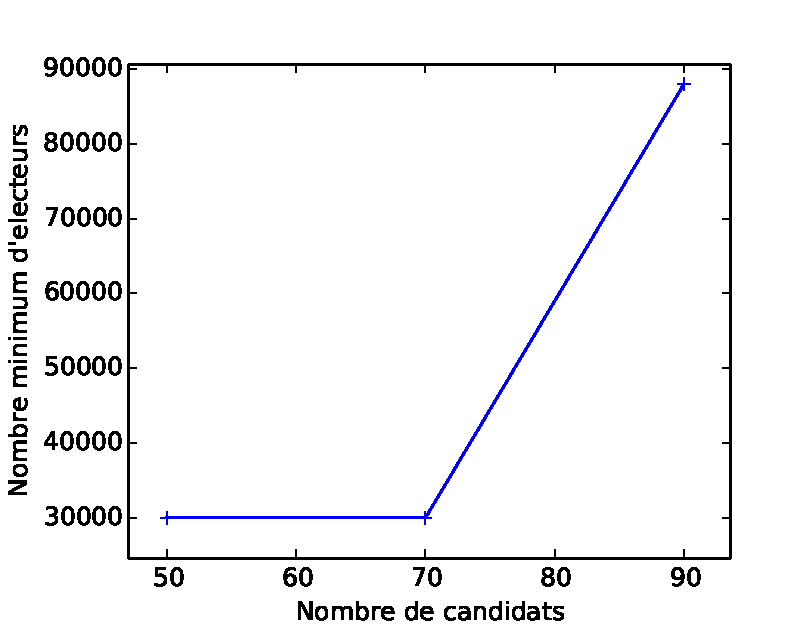
\includegraphics[width=0.98\columnwidth]{../\rootPath image/Nmin-electeurs.pdf}
  \caption{Le nombre minimal d'\'electeurs est donn\'e \`a 1000 \'electeurs pr\`es pour un nombre de candidats entre 50 et 90}
  \label{fig:minElecteurs}
\end{figure}

, 
\end{document}





\section{Conclusion}

Cet article pr\'esente le syst\^eme de vote de laPrimaire.org. En construisant judicieusement des lots de candidats, nous avons montr\'e que le classement du vote est le m\^eme lorsque les \'electeurs votent pour ces lot plut\^ot que pour tous les candidats. 





%%=============================================================================
%%=============================================================================
\ifstandalone
	\bibliographystyle{IEEEtran}
	\bibliography{\rootPath Annexes/biblio.bib}
\fi
%%=============================================================================
%%=============================================================================

\end{document}
